\documentclass{beamer}

% For more themes, color themes and font themes, see:
% http://deic.uab.es/~iblanes/beamer_gallery/index_by_theme.html
%
\mode<presentation>
{
% Madrid is a good basic theme
%good themes: Antibes/dolphin, Boadilla/beaver/crane

  \usetheme{Antibes}       % or try default, Darmstadt, Warsaw, ... I like Singapore, 
  \usecolortheme{uiowa} % or try albatross, beaver, crane, ... I like seahorse, crane, or beaver
  \usefonttheme{serif}    % or try default, structurebold, ...
  \setbeamertemplate{navigation symbols}{}
  \setbeamertemplate{caption}[numbered]
  \setbeamertemplate{bibliography item}[text]
  %\setbeamercolor{titlelike}{fg=black, bg=white}
} 
\usepackage[english]{babel}
\usepackage[utf8x]{inputenc}
\usepackage{pgfpages}
\pgfpagesuselayout{resize to}[%
  physical paper width=8in, physical paper height=6in]


% Pacakges and commands that I like:
%For math symbols
\usepackage{amsmath} 
\usepackage{amsfonts}%
\usepackage{amssymb}
\usepackage{amsthm}
%\usepackage{titlesec}
%For Graphics
\usepackage{graphicx}
\usepackage{multicol}
\usepackage{subcaption}
%Setup Page
%\usepackage{fullpage} 
% \usepackage[margin=.5in]{geometry}
% \usepackage{fancyhdr}
% \pagestyle{fancy}
% \setlength{\headheight}{14pt}

\def \R{\ensuremath \mathbb{R}}
\def \e{\ensuremath \varepsilon}
\def \d{\ensuremath \delta}
\def \tr{\ensuremath \text{tr}}
\newcommand{\vect}[1]{\boldsymbol{#1}}

\theoremstyle{definition}
\newtheorem{defn}{Definition}[section]
\newtheorem{thm}{Theorem}[section]
\newtheorem*{cor}{Corollary}


%%%%%%%%%%%%%%%%%%%%%%%%%%%%%%%%%%%%%%%%%%%%%%%%%%%%%%%%%%%%%%%%%%%%%%%%%%%%%%
%%%%%%%%%%%%%%%%%%%%%%%%%%%%%%%%%%%%%%%%%%%%%%%%%%%%%%%%%%%%%%%%%%%%%%%%%%%%%%
% Here's where the presentation starts, with the info for the title slide
\title[Neural Network Methods for Application in Educational Measurement]{Neural Network Methods for Application \\ in Educational Measurement}
\author{Geoffrey Converse}
\institute{University of Iowa}
\date{July 15, 2021}

\begin{document}


\begin{frame}
  \titlepage
  \begin{center}
  {\scriptsize PhD Defense in Applied Mathematical and Computational Sciences}
  \end{center}
\end{frame}


\begin{frame}{Outline}
  \tableofcontents
\end{frame}

\begin{frame}{Acknowledgements}
  people
\end{frame}

\begin{frame}{Workspaces}
  pics of old office, mlh, work from home during covid, margot
\end{frame}

\section{Item Response Theory}

\begin{frame}{Item Response Theory (IRT)}
\begin{itemize}
  \item Goal: Explain relationship between student ability and exam performance
  \item Assume each subject has a latent ``ability'' value $\theta$
  \begin{itemize}
    \item<2-> $\theta$ is not directly observable
    \item<2-> Often assume $\theta \sim \mathcal{N}(0,1)$
    \item<2-> Naive solution: accuracy (percent correct)
  \end{itemize}
  \item<3> For an assessment with $n$ items taken by $N$ subjects, what is the probability that student $j$ answers item $i$ correctly?
  \[P(u_{ij}=1 | \theta_j) = f(\theta_j; V_i)\]
  \begin{itemize}
    \item<3> $\theta_j =$ latent ability of subject $j$
    \item<3> $V_i =$ set of parameters associated with item $i$
  \end{itemize}
\end{itemize}
\end{frame}

\begin{frame}{Rasch Model}
\begin{itemize}
  \item Define $\d_i > 0$ as the difficulty of item $i$, and $\eta_j > 0$ the ability of subject $j$.
  \item Rasch: Probability of success depends on ratio $\zeta_{ij} = \frac{\eta_j}{\d_i}$
  \[P(u_{ij} = 1 | \zeta_{ij}) = \frac{\zeta_{ij}}{1 + \zeta_{ij}} = \frac{\eta_j}{\eta_j + \d_i}\]
  \item Logarithmic transformation: $\theta_j = \log \eta_j$ and $\beta_i = \log \d_i$
  \item Rasch Model :
  \[P(u_{ij} = 1 | \zeta_{ij}) = \frac{1}{1 + e^{\beta_i - \theta_j}}\]
\end{itemize}
\end{frame}

\begin{frame}{2-Parameter Logistic Model (2PL)}
\begin{itemize}
  \item Probability of a correct response follows the logistic equation:
  \[P(u_{ij} = 1 | \theta_j) = \frac{1}{1 + e^{-a_i(\theta_j - b_i)}}\]
  \begin{itemize}
    \item<2-> Scaling $a_i$ by a factor of 1.7 makes 2PL differ from the normal ogive by $<0.01$ uniformly
    \item<2-> Easier to compute than normal ogive
    \item<2-> $a_i =$ discrimination parameter
    \item<2-> $b_i =$ difficulty parameter
  \end{itemize}
\end{itemize}
\end{frame}

\begin{frame}{Item Characteristic Curve (ICC)}
\begin{figure}
  \includegraphics[width=.7\textwidth]{../img/logistic_2param_icc.jpg}
\end{figure}

\end{frame}
\begin{frame}{Multidimensional IRT}
\begin{itemize}
  \item Now assume that an assessment is testing $K$ skills
  \begin{itemize}
    \item For example, a math exam can test skills add, subtract, multiply, divide
    \item Each student has a vector of skills $\Theta_j = (\theta_{j1},.., \theta_{jK})^T$
    \item Multiple skills can be assessed by a single item
  \end{itemize}
  \item<2-> Binary $Q$-matrix defines relationship between items and skills
  \begin{itemize}
    \item<2-> $Q \in \R^{n \times K}$, \[q_{ik} = \begin{cases}
    1 & \text{if item } i \text{ requires skill } k \\ 
    0 & \text{otherwise} 
    \end{cases}\]
  \end{itemize}
\end{itemize}
\end{frame}

\begin{frame}{Multidimensional Logistic 2-Parameter (ML2P) Model}
\begin{itemize}
\item Probability of correct response given by:
  \[P(u_{ij}=1 | \Theta_j) = \frac{1}{1 + \exp[-\sum_{k=1}^K a_{ik}\theta_{jk} + b_i]}\]
  \begin{itemize}
    \item<2-> $a_{ik} =$ discrimination parameter between item $i$ and skill $k$ 
    \item<2-> $b_i =$ difficulty parameter
  \end{itemize}
\end{itemize}
\end{frame}

\subsection{IRT Parameter Estimation Methods}

\begin{frame}{Joint Maximum Likelihood Estimation (JMLE)}
\begin{itemize}
  \item Need to estimate student and item parameters simultaneously
  \item<2-> $N$ students and $n$ items, build $n\times N$ response matrix $[u_{ij}]$ and ability vector $\Theta = (\theta_1,...,\theta_N)^T$
  \item<2-> Probability of item responses:
  \[P(U|\Theta) = \prod_{j=1}^N \prod_{i=1}^n P_{ij}^{u_{ij}} (1-P_{ij})^{1-u_{ij}}\]
  \item<3> Maximize log-likelihood:
  \[L = \log P(U|\Theta) = \sum_{j=1}^N \sum_{i=1}^n u_{ij} \log P_{ij}  + (1-u_{ij}) \log (1-P_{ij})\]
\end{itemize}
\end{frame}

\begin{frame}{Joint Maximum Likelihood Estimation (JMLE)}
\begin{itemize}
  \item Maximizing log-likelihood gives $2n+N$ equations.
  \item Using Newton's Method: $A_{t+1} = A_t - B_t^{-1}F_t$
  \begin{itemize}
    \item $A = (\hat a_1, \hat b_1, ..., \hat a_n, \hat b_n, \hat\theta_1, ..., \hat\theta_N)^T$ vector of estimates 
    \item $B = $ $(2n+N) \times (2n+N)$ matrix of 2nd order partials
    \item $F = $ vector of 1st order partials
  \end{itemize}
  \item<2-> Assumptions:
  \begin{itemize}
    \item<2-> Each examinee is independent
    \item<2-> Items are independent
    \item<2-> Examinees and items are independent
  \end{itemize}
  \item<3> Simplification: Assume most cross-derivatives are zero
\end{itemize}
\end{frame}

\begin{frame}{Are examinees and items really independent?}
  TODO: calculate item/examinee cross-derivatives %TODO
\end{frame}

\begin{frame}{JMLE Jacobian Matrix}
  TODO: change this to multidimensional (blocks A,B,C,t(B))
\[B = \begin{bmatrix}
\frac{\partial^2L}{\partial a_1^2} & \frac{\partial^2L}{\partial a_1 b_1} & & & & & & & \\
\frac{\partial^2L}{\partial a_1 b_1} & \frac{\partial^2L}{\partial b_1^2} & & & & & & & \\
& & \ddots & & & & & & \\
& & & \frac{\partial^2L}{\partial a_n^2} & \frac{\partial^2L}{\partial a_n\zeta_n} & & & & \\
& & & \frac{\partial^2L}{\partial a_n b_n} & \frac{\partial^2L}{\partial b_n^2} & & & & \\
& & & & & \ddots & & & \\
& & & & & & \frac{\partial L^2}{\partial \theta_1^2} & & \\
& & & & & & & \ddots & \\
& & & & & & & & \frac{\partial L^2}{\partial \theta_N^2} 
\end{bmatrix}\]
\end{frame}

\begin{frame}{JMLE Difficulties}
\begin{itemize}
  \item Need good initial ability estimates
  \item Possibly unbounded $a_i$, $b_i$, and $\theta_j$ estimates
    \begin{itemize}
      \item If student $j$ answers all items correctly: $\hat \theta_j \to \infty$
      \item If nobody answers item $i$ correctly: $\hat b_i \to -\infty$
    \end{itemize}
  \item Solution can diverge
  \begin{itemize}
    \item Large discrimination parameter estimates can lead to large ability estimates
  \end{itemize}
\item Large matrix inversions
\end{itemize}
\end{frame}

\begin{frame}{Marginal Maximum Likelihood (MMLE)}
\begin{itemize}
  \item Assume that $\theta$ follows some distribution $g(\theta)$
  \item Maximize the mariginal likelihood for each student
  \[P(U_j) = \int P(U_j | \theta) g(\theta) d\theta\]
  \item<2-> Marginal likelihood function
  \[L = \prod_{j=1}^N P(U_j) = \prod_{j=1}^N \int P(U_j | \theta) g(\theta) d\theta\]
  \item<3-> Posterior probability
  \[P(\theta_j | U_j) = \frac{P(U_j | \theta_j) g(\theta_j)}{P(U_j)} = \frac{P(U_j | \theta_j) g(\theta_j)}{\int P(U_j | \theta) g(\theta) d\theta}\]
\end{itemize}
\end{frame}

\begin{frame}{Marginal Maximum Likelihood (MMLE)}
  \begin{align*}
  \frac{\partial \log L}{\partial x_i}  &= \sum_{j=1}^N \frac{1}{P(U_j)} \int \frac{\partial}{\partial x_i} [P(U_j |\theta)] g(\theta) d\theta \\
  \onslide<2->{&= \sum_{j=1}^N \frac{1}{P(U_j)} \int \frac{\partial}{\partial x_i} [\log P(U_j |\theta)] P(U_j |\theta) g(\theta) d\theta} \\
  \onslide<3->{&= \sum_{j=1}^N \int \frac{\partial}{\partial x_i} [\log P(U_j |\theta)] P(\theta | U_j) d\theta} \\
  \onslide<4->{\frac{\partial \log L}{\partial a_i} &= \sum_{j=1}^N \int (\theta - b_i) (u_{ij} - P_{ij})P(\theta|U_j) d\theta \\
  \frac{\partial \log L}{\partial b_i} &= -a_i\sum_{j=1}^N \int(u_{ij} - P_{ij})P(\theta|U_j) d\theta}
  \end{align*}
\end{frame}

\begin{frame}{MMLE}
  quadrature or mcmc - difficult for high dim theta
\end{frame}



\section{Neural Networks}

\begin{frame}{Artificial Neural Networks (ANN)}
\begin{center}
  \includegraphics[width=.55\textwidth]{../img/ffn_visual.png}
Input $\vect x$, approximate a true target $\vect y$ via a series of (learned) linear transformations and nonlinear re-scaling
\[\hat{\vect y} = \sigma(W_3\sigma(W_2\sigma(W_1 \vect x + vect b_1) + \vect b_2) + \vect b_3)\]
Learn $W_l$ and $\vect b_l$ via gradient descent
\end{center}
\end{frame}

\subsection{Autoencoders}

\begin{frame}{Autoencoder (AE)}
\begin{itemize}
  \item Encode data into smaller dimension
  \item Reconstruct original input
\end{itemize}
  TODO: make AE image using NN SVG and show MNIST reconstruct example
\end{frame}

\subsection{Variational Autoencoders}
\begin{frame}{Variational Autoencoder (VAE)}
\begin{itemize}
\item Commonly used as a generative neural network
\item Learn a low-dimensional latent representation $\theta$ which is capable of generating original data $x$ from some distribution
\[
f(\boldsymbol{\theta} | \boldsymbol{x})=\frac{P(\boldsymbol{X}=\boldsymbol{x}| \theta) f(\boldsymbol{\theta})}{P(\boldsymbol{X}=\boldsymbol{x})}
\]
\begin{equation}\label{marginal}
{P(\boldsymbol{X}=\boldsymbol{x})=\int P(\boldsymbol{X}=\boldsymbol{x}| \boldsymbol{\theta}) f(\boldsymbol{\theta})d\boldsymbol{\theta}},\nonumber
\end{equation}
\item<2-> Approximate $f(\boldsymbol{\theta} | \boldsymbol{x})$ with some $q(\boldsymbol{\theta} | \boldsymbol{x})$ $\Rightarrow$ minimize KL Divergence
\end{itemize}
\end{frame}

\begin{frame}{Kullback-Leibler Divergence}
\begin{itemize}
  \item<1-> \textit{Entropy} measures average information gained from 1 sample:
  \[H(P) = \mathbb{E}_P[-\log P(x)] =  - \sum_i P(x_i) \log P(x_i)\]
  \item<2-> \textit{Cross entropy} measures average information needed when using approximate distribution $Q(x)$ instead of true distribution $P(x)$:
  \[H(P,Q) = \mathbb{E}_P[-\log Q(x)] = -\sum_i P(x_i) \log Q(x_i)\]
  \item<3-> \textit{Kullback-Leibler Divergence} measures difference between two probability distributions $P(x)$ and $Q(x)$:
\[\mathcal{D}_{KL} \left[ P(x) || Q(x) \right] = H(P,Q) - H(P) = \sum_i P(x_i) \log \left(\frac{P(x_i)}{Q(x_i)} \right)\]
%   \item Between an independent, $k$-dimensional, multivariate normal distribution and $\mathcal{N}(0, I)$:
% \begin{align*}
% \mathcal{D}_{KL} \left[\mathcal{N}(\mu, \sigma^2) || \mathcal{N}(0, I) \right] = \frac{1}{2} \sum_{i=1}^k (\sigma_i^2 + \mu_i^2 - \ln(\sigma_i^2) - 1)
% \end{align*}
\end{itemize}
\end{frame}

\begin{frame}{VAE loss}
  TODO: derive VAE loss
\end{frame}

\begin{frame}{Variational Autoencoder (VAE)}
\begin{figure}
  \includegraphics[width=.7\textwidth]{../img/vae_visual.png}
\end{figure}
\begin{itemize}
  \item<1-> Fit encoded space to a normal distribution
  \begin{itemize}
    \item<1-> Loss funcion: $L(x) = L_0(x) + KL[q_\alpha(\theta | x) || \mathcal{N}(0,I)] $
  \end{itemize}
  \item<2-> Sample $\e \sim \mathcal{N}(0,1)$, set $z = \mu + \sigma \e$
\end{itemize}
\end{frame}

\begin{frame}{Variational Autoencoder (VAE)}
  mona lisa visual might be okay, but want to emphasize that encoder learns a posterior distribution
%\begin{figure}
%\includegraphics[width=.8\textwidth]{img/vae_dist/combined.png}
%\end{figure}
\end{frame}

\section{ML2P-VAE for Parameter Estimation}

\begin{frame}{Combining IRT and ANN}
\begin{itemize}
  \item Key similarities:
  \begin{itemize}
    \item IRT and VAE assume normally distributed latent space
    \item<2-> ML2P model and sigmoidal activation function:
  \end{itemize}
  \begin{align*}
  \onslide<2->{
  P(u_{ij}=1 | \Theta_j) &= \frac{1}{1 + \exp[-\sum_{k=1}^K a_{ik}\theta_{jk} + b_i]} \\
  \sigma(z) = \sigma(\vec{w}^T \vec{a} + b) &= \frac{1}{1 + \exp[-\sum_{k=1} w_k a_k - b]}}
  \end{align*}

\end{itemize}
\end{frame}

\subsection{ML2P-VAE Method}

\begin{frame}{Model Description}
\begin{itemize}
\item No hidden layers in the decoder
\item<2-> Restrict nonzero weights in the decoder according to $Q$-matrix
\item<3-> Sigmoidal activation function in output layer
\item<4-> Require decoder weights to be nonnegative
\item<5-> Fit VAE latent space to $\mathcal{N}(0, I)$
\item<6-> Decoder interpreted as the ML2P model
  \begin{itemize}
    \item<6-> Activation of nodes in learned distribution $\Rightarrow$ latent skills
    \item<6-> Weights in decoder $\Rightarrow$ discrimination parameters
    \item<6-> Bias of output nodes $\Rightarrow$ difficulty parameters
  \end{itemize}
\end{itemize}
\end{frame}

\begin{frame}{ML2P-VAE}
\begin{center}
  \includegraphics[scale=0.45]{../img/ml2pvae_visual.png}
\end{center}
\end{frame}

\begin{frame}{ML2P-VAE Testing}
\begin{itemize}
  \item Testing
  \begin{itemize}
    \item Simulated 28 item assessment with 3 latent skills and pre-determined $Q$-matrix 
    \begin{itemize}
      \item Discrimination and difficulty parameters randomly chosen 
    \end{itemize}
    \item $N$ subjects with latent skills drawn from $N(0,I)$
    \item<2-> For each student $j$:
    \begin{itemize}
      \item<2-> For each item, calculate probability of success $P_{ij}$ from ML2P model
      \item<2-> Sample from these probabilities to generate response set $U_j = (u_{j,1},...u_{j,28})$
    \end{itemize}
  \end{itemize}
  \item<3-> Results presented at International Joint Conference on Neural Networks (IJCNN) 2019
\end{itemize}
\end{frame}

\begin{frame}{ML2P-VAE Results}
\begin{center}
\scriptsize

Relative Error\\
\begin{tabular}{ccccc}
% \hline
% &&&&\\
\hline
Size  & $a_1$ & $a_2$ & $a_3$ & $b$ \\
\hline
500   & 0.779 & 0.699 & 0.759 & 1.188 \\
5,000 & 0.539 & 0.281 & 0.585 & 1.673 \\
10,000  &0.284  & 0.159 & 0.264 & 1.894 \\
\hline
\end{tabular}

\vspace{.5cm}

Root Mean Square Error\\
\begin{tabular}{ccccc}
% \hline
% &&&&\\
\hline
Size  & $a_1$ & $a_2$ & $a_3$ & $b$   \\
\hline
500   & 0.976 & 0.931 & 0.850 & 1.038 \\
5,000 & 0.587 & 0.823 & 0.414 & 1.494 \\
10,000  & 0.322 & 0.346 & 0.264 & 1.670 \\
\hline
\end{tabular}

\vspace{.5cm}

Correlation\\
\begin{tabular}{ccccc}
% \hline
% &&&&\\
\hline
Size  & $a_1$ & $a_2$ & $a_3$ & $b$ \\
\hline
500   & 0.457 & 0.547 & 0.381 & 0.987 \\
5000  & 0.779 & 0.710 & 0.990 & 0.982 \\
10000   & 0.924 & 0.920 & 0.986 & 0.990 \\
\hline
\end{tabular}
\end{center}
\end{frame}

\begin{frame}{ML2P-VAE Results}
\begin{figure}[h!]
\minipage{0.45\textwidth}
\includegraphics[width=\textwidth]{../img/ijcnn_results/10k_a.eps}
\endminipage\hfill
\minipage{0.45\textwidth}
\includegraphics[width=\textwidth]{../img/ijcnn_results/10k_b.eps}
\endminipage\hfill
% \caption{Autoencoder and VAE discrimination parameter ($a_{ji}$) recovery.}
% \label{fig:a_corr}
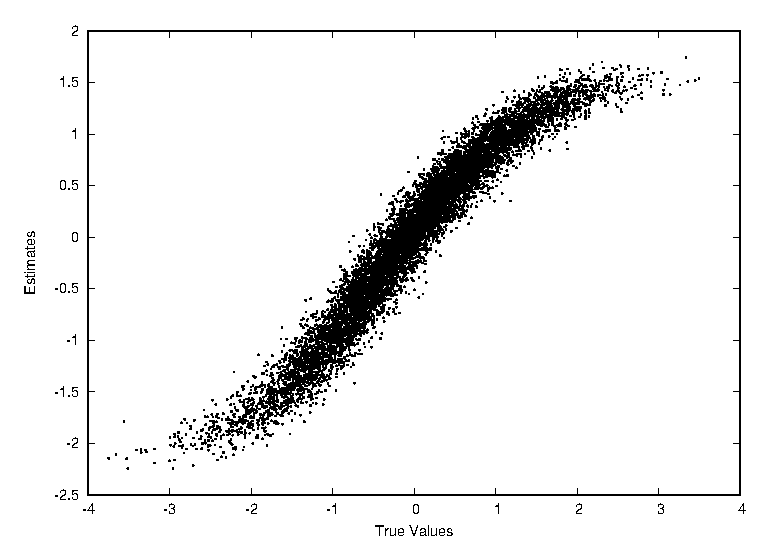
\includegraphics[width=.45\textwidth]{../img/ijcnn_results/10k_t1_scaled.eps}
% \caption{test caption}
% \label{f}
\end{figure}
\end{frame}


\subsection{Why use a \textit{Variational} Autoencoder?}

\begin{frame}{VAE vs AE Comparison}
\begin{itemize}
  \item Guo, Cutumisu, and Cui proposed using AE in skill estimation
  \item Directly compare neural networks in ML2P application
  \begin{itemize}
    \item Parameter recovery
    \item Skill estimation
  \end{itemize}
  \item<2-> Results presented at Artificial Intelligence in Education (AIED) 2019
\end{itemize}
\end{frame}

%%%% Include tables or no?
% \begin{frame}{VAE vs AE Comparison}
% \begin{table}[h]
%     \centering
%     \begin{tabular}{ccccc}
% \hline
% Model & $\theta_1$ & $\theta_2$ & $\theta_3$ & Statistic \\
% \hline
% AE &  7.425 & 3.107 & 16.260 & AVRB \\
% VAE   & 1.844 & 1.713 & 4.009 &  \\
% \hline
% AE & 1.788 & 1.523 & 1.746 & RMSE \\
% VAE   & 0.664 & 0.760 & 0.646 & \\
% \hline
% AE & 0.970 & 0.937 & 0.971 & CORR \\
% VAE   & 0.965 & 0.940 & 0.969 & \\
% \hline
%     \end{tabular}
%     \caption{Statistics for latent trait prediction with data size $n=10,000$.}
%     \label{tab:theta_stats}
% \end{table}
% \end{frame}

\begin{frame}{VAE vs AE Comparison}
\begin{figure}[h!]
\minipage{0.39\textwidth}
\includegraphics[width=\textwidth]{../img/aied_results/ae_a_corr.png}
\endminipage\hfill
\minipage{0.39\textwidth}
\includegraphics[width=\textwidth]{../img/aied_results/vae_a_corr.png}
\endminipage\hfill
% \caption{Autoencoder and VAE discrimination parameter ($a_{ji}$) recovery.}
% \label{fig:a_corr}

\minipage{0.39\textwidth}
\includegraphics[width=\textwidth]{../img/aied_results/ae_b_corr.png}
\endminipage\hfill
\minipage{0.39\textwidth}
\includegraphics[width=\textwidth]{../img/aied_results/vae_b_corr.png}
\endminipage\hfill
\caption{Autoencoder (left) and VAE (right) parameter recovery for discrimination parameters $a_{ij}$ (top) and difficulty parameters $b_i$ (bottom).}
\label{fig:b_corr}
\end{figure}
\end{frame}

\begin{frame}{VAE vs AE Comparison}
\begin{figure}
\minipage{0.39\textwidth}
\includegraphics[width=\textwidth]{../img/aied_results/ae_theta1_corr.png}
\endminipage\hfill
\minipage{0.39\textwidth}
\includegraphics[width=\textwidth]{../img/aied_results/vae_theta1_corr.png}
\endminipage\hfill
\end{figure}
\begin{itemize}
  \item Similar skill estimate correlation, but on different scale
  \item VAE much more accurate parameter recovery
\end{itemize}
\end{frame}


\subsection{Generalizing to Correlated Latent Traits}

\begin{frame}{Correlated Latent Traits in IRT}
\begin{itemize}
  \item In real applications, independent skills are not realistic: $\vect \Theta \sim \mathcal{N}(\vect \mu, \Sigma)$, not $\mathcal{N}(0,I)$.
  \begin{itemize}
    \item Example: students who are good at adding are also good at subtracting
  \end{itemize}
  \item<2-> Covariance matrix is symmetric, positive definite matrix
  \[\Sigma = \begin{bmatrix}
  \sigma_1^2 & c_{12} & \cdots & c_{1k} \\
  c_{21} & \sigma_2^2 & \cdots & c_{2k} \\
  \vdots & & \ddots & \vdots \\
  c_{k1} & \cdots & c_{k(k-1)} & \sigma_k^2
  \end{bmatrix}\]
  \item<2-> With variances $\sigma_i^2$ and covariances $c_{ij} = c_{ji}$
\end{itemize}
\end{frame}

\begin{frame}{Correlated Latent Code in VAE}
\begin{itemize}
  \item In most VAE applications, it is convenient to assume latent code $\vect z$ is \textit{independent}
    \begin{itemize}
      \item Forces each dimension of $\vect z$ to measure different features
      \item $\vect z$ is \textit{abstract}, with \textbf{no real-world understanding}
    \end{itemize}
  \item For ML2P-VAE, we know that latent code $\vect z$ approximates latent traits $\vect \Theta$
    \begin{itemize}
      \item We may have \textbf{domain knowledge} of the distribution of $\vect \Theta$
    \end{itemize}
\end{itemize}
\end{frame}

\begin{frame}{A novel VAE architecture for correlated latent code}
  
\end{frame}

\begin{frame}{Correlated Latent Code in VAE}
\begin{itemize}
  \item KL Divergence between two $k$-dimensional multivariate normal distributions:
\begin{align*}
&\mathcal{D}_{KL}\left[\mathcal{N}(\mu_0, \Sigma_0) || \mathcal{N}(\mu_1, \Sigma_1)\right] = \\
&\frac{1}{2} \left(\tr(\Sigma_1^{-1} \Sigma_0) + (\mu_1 - \mu_0)^T \Sigma_1^{-1} (\mu_1 - \mu_0) - k + \ln\left(\frac{\det \Sigma_1}{\det \Sigma_0} \right) \right)
\end{align*}
  \item<2-> When fitting a VAE, $\mathcal{N}(\mu_1, \Sigma_1)$ is known, so $\mu_1$ and $\Sigma_1$ are constant
  \item<2-> $\mu_0$ and $\Sigma_0$ obtained from feeding one sample through the encoder
\end{itemize}
\end{frame}

% \begin{frame}{Full Covariance Matrix in VAE}
% picture of full covariance VAE architecture
% \[\mu_0 = (m_1, m_2)^T\]
% \[L_0 = \begin{bmatrix}
% a_{11} & 0 \\ a_{21} & a_{22}
% \end{bmatrix}\]
% \end{frame}

\begin{frame}{Correlated VAE Implementation}
\begin{itemize}
  \item To sample from a multivariate normal distribution $\mathcal{N}(\mu_0, \Sigma_0)$:
  \begin{itemize}
    \item Find a matrix $G$ such that $G G^T = \Sigma_0$
    \item Sample $\e = (\e_1,...,\e_k)^T$ with each $\e_i \sim \mathcal{N}(0,1)$
    \item Generate sample $z = \mu_0 + G\e$
  \end{itemize}
  \item<2-> KL Divergence calculation uses $\mu_0$, $\Sigma_0$, and requires $\det \Sigma_0 > 0$
\end{itemize}
\begin{figure}
  \onslide<3->{\includegraphics[width=.7\textwidth]{../img/ml2pvae_visual.png}
\caption*{Encoder structure for VAE learning $\mathcal{N}(0,I)$}}
\end{figure}
\end{frame}

\begin{frame}{Correlated VAE Implementation}
\begin{itemize}
  \item Architecture: Encoder outputs $k + k(k+1)/2$ nodes
  \begin{itemize}
    \item $k$ nodes for $\mu_0$, and $k(k+1)/2$ nodes for $L_0$ lower triangular
  \end{itemize}
  \item<2-> Sampling: Calculate $G_0 = e^{L_0}$ 
  \begin{itemize}
    \item<2-> Note $G_0$ is lower triangular, nonsingular
    \item<2-> Send sample $z = \mu_0 + G_0\e$ through decoder
  \end{itemize}
  \item<3-> KL Divergence: Calculate $\Sigma_0 = G_0 G_0^T$
  \begin{itemize}
    \item<3-> Note that
  \begin{align*}
  \det\Sigma_0 &= \det (e^{L_0} (e^{L_0})^T) = \det e^{L_0} \cdot \det (e^{L_0})^T \\
  &= e^{\tr {L_0}} \cdot e^{\tr {L_0}^T} = \left(e^{\tr {L_0}}\right)^2 \\
  &> 0
  \end{align*}
    \item<4-> Claim: $\Sigma_0$ is symmetric positive definite
  \end{itemize}
\end{itemize}
\end{frame}

\begin{frame}{Correlated VAE Implementation}
\textbf{Claim}: $\Sigma_0$ is symmetric and positive definite.
\begin{proof}
\small
For each sample $x_0$, the encoder returns $L_0 \in \R^{k \times k}$ lower triangular. \onslide<2->{Consider the matrix exponential 
\[G_0 := e^{L_0} = \sum_{n=0}^\infty \frac{L_0^n}{n!} = I + L_0 + \frac{1}{2}L_0^2 + \cdots\]}
\onslide<3->{$G_0$ is lower triangular, since addition and multiplication preserve lower triangular. $G_0$ is also nonsingular: 
\[\det G_0 = \det e^{L_0} = e^{\tr L_0} \not = 0\]}
\onslide<4->{Set $\Sigma_0 := G_0 G_0^T$. Now for any nonzero $y \in \R^k$,}
\onslide<5->{\[\langle \Sigma_0y, y \rangle = y^T \Sigma_0 y = y^T G_0 G_0^T y = \langle G_0^T y, G_0^T y \rangle = ||G_0^T y||_2^2 > 0\]}
\end{proof}
\end{frame}


\subsection{R Package}
\begin{frame}{Package in R}
\begin{itemize}
  \item Create software package in R with ML2P-VAE method
  \item Submit to CRAN for resarchers without tensorflow experience to use
  \item<2-> Package functions:
  \begin{itemize}
    \item<2-> Construct ML2P-VAE model to desired architecture
    \item<2-> Option for independent latent traits, or full covariance matrix
    \item<2-> Sufficient documentation and working examples
  \end{itemize}
\end{itemize}
\end{frame}



\section{Knowledge Tracing}
\begin{frame}{Temporal Neural Networks}
  RNN, LSTM, Transformers
\end{frame}


\section{}
\begin{frame}{References}
\begin{thebibliography}{2}
\tiny

\bibitem{thissen} Wainer and Thissen, D. ``Test Scoring''. Erlbaum Associates, Publishers, 2001.

\bibitem{dasilva} da Silva, Liu, Huggins-Manley, Bazan. ``Incorporating the Q-matrix into Multidimensional Item Response Models.'' Journal of Educational and Psychological Measurement, 2018.

\bibitem{baker} Baker and Kim. ``Item Response Theory: Parameter Estimation Techniques''. CRC Press, 2004.

\bibitem{bock} Bock and Aitken. ``Marginal Maximum Likelihood Estimation of Item Parameters: Application of an EM Algorithm''. Psychometrika, 1981.

\bibitem{nielsen} Nielsen, Michael. ``Neural Networks and Deep Learning''. Determination Press, 2015.

\bibitem{ijcnn} Curi, Converse, Hajewski, Oliveira. ``Interpretable Variational Autoencoders for Cognitive Models.'' In Proceddings of the International Joint Conference on Neural Networks (IJCNN), 2019.

\bibitem{guo} Q. Guo, M. Cutumisu, and Y. Cui. ``A Neural Network Approach to Estimate Student Skill Mastery in Cognitive Diagnostic Assessments''. In: 10th International Conference on Educational Data Mining. 2017.

\bibitem{aied} Converse, Curi, Oliveira. ``Autoencoders for Educational Assessment.'' In Proceedings of the Conference on Artifical Intelligence in Education (AIED), 2019.

\bibitem{fsdm} Converse, Curi, Oliveira, and Arnold. ``Variational Autoencoders for Baseball Player Evaluation.'' In Proceedings of the Fuzzy Systems and Data Mining Conference (FSDM), 2019.  


\end{thebibliography}
\end{frame}

\begin{frame}
  \titlepage
\end{frame}

\end{document}
